\documentclass{article}

% biblio stuff
\usepackage[
backend=biber,
%style=alphabetic,
sorting=ynt
]{biblatex}

% update this to whatever the bibliography file is
\addbibresource{references.bib}

%%% title and whatnot %%%

\title{Meta-analysis of Medians}

\author{Charles T. Gray, Luke Prendergast, Emily Kothe, and Hien Nguyen\thanks{
The authors are appreciative for the insights and comments from Kerrie Mengersen, and Kate Smith-Miles.
}}

%todo ask kate & kerrie how they'd like to be acknowledged

%%% packages and macros

%% always load packages

\usepackage{amsmath, amssymb}
\usepackage{booktabs}
\usepackage[utf8]{inputenc}
\usepackage{csquotes}
\usepackage[english]{babel}


%%% macros

% code macro
\newcommand{\code}[1]{\texttt{#1}}
\newcommand{\package}[1]{\texttt{#1::}}

% more words macro
\usepackage{todonotes}
\newcommand{\morewords}[1]{
    \todo[inline, color=lightgray]{\footnotesize{\textbf{more words} #1}}
}
\newcommand{\dothislater}[1]{
    \todo[color=gray]{\footnotesize{\textbf{do this later} #1}}
}


% stats macros
\DeclareMathOperator{\var}{var}
\DeclareMathOperator{\iqr}{iqr}
\newcommand{\preimage}[1]{#1^{-1}}
\DeclareMathOperator{\varmed}{varmed}

% bold math
\usepackage{bm}

% theorerm macros
\newtheorem{disadv}{Disadvantage}
\newtheorem{remark}{Remark}


%%% doc %%%

\begin{document}

\maketitle

%%% abstract %%%

\begin{abstract}
  % todo: abstract
\end{abstract}

%%% main text %%%

\section{Medians pose a problem in meta-analyses}

Software tools for meta-analysis, such as Cochrane's
RevMan~\cite{reviewmanagerRevMan}, newly superseded by the cloud-based RevMan Web~\cite{reviewmanagerRevManWeb}
or the R package \package{metafor}~\cite{viechtbauerConductingMetaanalysesMetafor2010},
require estimates of both effect and variance
of that effect. However, the sample variance for the reported effect of interest is not always available.
When the reported statistics are medians, measure of spreads commonly provided are in the form of quartiles, as opposed to the required variance of the effect of interest. This leads to the omission of studies that report medians from the meta-anaysis. In this manuscript we present a method for estimating the variance of the sample median so that studies reporting medians may be included in meta-analyses.

This manuscript is a component of the research compendium created to solve this problem. In this case, the research compendium comprises not just a manuscript, but a pair of software packages, \package{varameta}~\cite{grayVarametaEstimatorsVariance2020}, which translates estimators presented in this manuscript to code, and \package{simeta}~\cite{graySimetaSimulateMetaanalysis2020}, for simulating meta-analysis data, to see how the estimators in \package{varameta} perform. Thus, in addition to intrinsic questions regarding meta-analysing medians, this manuscript considers on the ideas presented in the companion papers~\cite{gray2019textttcodeproof, grayTruthProofReproducibility2019} that ruminate, with this analysis as a case study, on why and how we may build reproducible research compendia.

\subsection{What's the problem?}

In published research, skewed data is often summarised by reporting the median and interquartile range. While this may be useful in a descriptive single-study sense, the lack of reported estimator variability poses a challenge in the context of meta-analysis.  Software for performing meta-analyses, such as the widely-used \texttt{R} package \package{metafor}~\cite{viechtbauerConductingMetaanalysesMetafor2010}, require an estimate of the variance of the reported effects to conduct the meta-analysis under the assumed model

\begin{equation}
\widehat{\delta}_k=\delta + \gamma_k + \varepsilon_k
\end{equation}
where $\widehat{\delta}_k$ is the estimated effect from the $k$th study, $\delta$ is the population effect of interest, $\varepsilon_k$ is the error allowing for sampling variability and $\gamma_k\sim N(0,\tau^2)$ is the random effect to allow for differences in the true effects between studies.  Given the estimated effects for $K$ studies, all assumed to be normally distributed with a known (or estimated) variance, a meta-analysis can be carried out to estimate $\delta$ and the random effect variance $\tau^2$.  Our focus is on meta-analysis of three different effects involving the median.  The first is simply the median itself when there is only one group of interest in each study.  The second is the difference of two medians when there is two groups to be compared within each study (such as a case and control group).  The third, which may be more suitable than the difference in medians when measurements of scale differ between studies, is the ratio of medians.   For more on meta-analysis see, e.g.,~\cite{borenstein2008introduction} and~\cite{kulinskaya2008meta}.

\subsection{Why propose a new method?}

In this paper we propose a method for meta-analyses of studies whose effects are reported in the form of median and interquartile range (or range). The previously proposed method of~\cite{hozoEstimatingMeanVariance2005}, and extensions by~\cite{blandEstimatingMeanStandard2014, wanEstimatingSampleMean2014}, solve this problem by estimating the mean and standard deviation from the provided summary statistics. For some applications there may be two noticeable drawbacks to this approach.

\begin{disadv}\label{disadv:1}
The methods to convert to a mean and standard deviation perform well when the underlying distribution is symmetric, and in some cases more specifically when it is normal.  However, results have shown that performance can be poor in the presence of skew (e.g., see~\cite{shi2018estimate}).
\end{disadv}

\begin{disadv}\label{disadv:2}
Those initially who published the summary measures, may have chosen to report medians and ranges because they had decided that moment-based measures such as the mean were not suitable descriptors.
\end{disadv}

In the presence of underlying skewed distributions, both Disadvantages 1 and 2 may cause a real threat to the validity of any inference following conversion from

\dothislater{Ask to Hien & Luke about this.}
% provide defintion quantiles measures to moment-based measures.

The method that we propose can be easily adapted to both single-study and meta-analysis contexts.  In the case of meta-analyses, meta-regression may also be conducted when some of the studies report means and standard deviations and others report medians and interquartile ranges.  This can be done by introducing a moderator factor variable to explain the differences between an effect based on means and an effect based on medians.

To illustrate this problem, we begin with an example meta-analysis from medical research. We then briefly touch on how our method contributes to the existing solutions for this problem. In Section \ref{sec: var est}, we define our estimator for the variance of the sample median and consider alternatives. We show how this estimator can be used in meta-analysis, and extend to meta-regression if the difference between the means and medians are of interest. Simulation results are provided in Section \ref{sec: sims} that assess the performance of our estimator in both the single-study and meta-analysis setting.   Finally, in Section \ref{sec: pin again}, we return to the motivating example, discussed in Section \ref{sec: motiv}, to demonstrate how our method can be applied. Concluding remarks are provided in Section \ref{sec: conclusion}.

\section{A motivating example}
\label{sec: motiv}

To motivate our method, we provide an example of the variety of summary statistics that can arise in meta-analyses. We shall return to this example in Section \ref{sec: pin again} to see how our method facilitates a meta-regression of all studies, rather than just the three studies originally considered which were based on means and standard deviations.

We choose notations similar to those used by Wan \emph{et al.}~\cite{wanEstimatingSampleMean2014}.  Define:
$a$, the minimum value;
$q_1$, the first quartile;
$m$, the median;
$q_3$, the third quartile;
$b$, the maximum value;
$n$, the sample size.  $\iqr$ denotes the interquantile range and this may be reported as an interval, i.e. $(q_1,q_3)$, or a width, i.e. $q_3-q_1$. We also let $\overline{x}$ and $s$ denote the sample mean and sample standard deviation respectively.  Later, we subscript such measures appropriately to identify different groups within studies, and in the example below this equates to, e.g., $m_c$ denoting the median for a control group and $m_t$ for the treatment group.

As an example of how studies collated in meta-analyses report these summary statistics differently, consider the dataset presented in Table \ref{tab: pinheiro}, taken from a systematic review of d-dimer in pre-eclampsia~\cite{pinheiroDdimerPreeclampsiaSystematic2012}. Ideally, one would want to perform a meta-analysis using the effects from all studies. However, estimator variance is only reported for three of the seven studies presented with the remaining studies reporting medians and ranges.

% Why is this table out of alignment?
\begin{table}[!htbp] \centering
  \small
\begin{tabular}{@{\extracolsep{5pt}} ccccccccc}
\\[-1.8ex]\hline
\hline \\[-1.8ex]
& & \multicolumn{3}{c}{Control group} & \multicolumn{3}{c}{Treatment group} & \\ \cline{3-5} \cline{6-8}
study & year & location & scale & $n_c$ & location & scale & $n_t$ &
\bf{reported} \\
\hline \\[-1.8ex]
Dusse &2003 & 1146.6 & 311.2 & 28 & 1263.8 & 411.9 & 43 & $\bm{\overline x, s}$  \\
Schjtlein &1997 & 1390.0 & 559.0 & 97 & 1545.0 & 849.5 & 200 & $\bm{\overline x, s}$  \\
Terao &1991 & 221.52 & 179.9 & 80 & 347.87 & 460.5 & 13 & $\bm{\overline x, s}$  \\
Catarino &2008 & 538.2 & (391.2, 822.8) & 42 & 448.5  & (313.0, 1091.3) & 44 & $\bm{m, (q_1, q_3)}$ \\
Bellart &1998 & 545.0 & 225.0 & 65 & 2090.0 & 1800.0 & 12 & $\bm{m, \iqr}$ \\
Heilmann &2007 & 1149.0 & 456.0 & 33 & 1623.6 & 932.9 & 111 & $\bm{m, \iqr}$ \\
He & 1997 & 183.0 & (110.0, 340.0) & 24 & 315.0 & (145.0, 1150.0) & 30 & $\bm{m, (a, b)}$\\
\hline \\[-1.8ex]
\end{tabular}
\caption{Data from a meta-analysis of d-dimer levels in pre-eclampsia presented by \cite{pinheiroDdimerPreeclampsiaSystematic2012}, measures of location and scale are varied: there are means and standard deviations; medians and interquartile ranges; quartiles; and medians and ranges. The types of estimates reported are listed in the final column denoted `reported'.}
  \label{tab: pinheiro}
\end{table}

Three studies (first authors Dusse, Schjtlein, and Terao) detailed in the table provide the sample mean, $\overline x$, and standard deviation, $s$. Two studies (Bellart and Heilmann) provide the sample median, $m$, and interquartile range, $\iqr$. One study (Catrino) provides the sample median, as well as the first and third quartiles, $q_1$ and $q_3$. Finally, one more study (He) provides the sample median and the minimum $a$ and maximum $b$ observed values. All studies provide the sample size $n$ and their respective estimates of location and scale for both the control and the pre-eclamptic groups.

In order to perform a meta-analysis via conventional methods, we require, at minimum, the studies' effect estimates, associated variances, and sample sizes. While full access to the raw data of each study would enable researchers to calculate the necessary sample variance for each study, there are many practical reasons, such as the time it would take to gather the data, that reduce the practicality of this approach, a point that is well made by others~\cite[e.g., p. 57]{blandEstimatingMeanStandard2014}.   Since only three studies presented in Table \ref{tab: pinheiro} report sample variance, Pinheiro \emph{et al.}'s meta-analysis was restricted to these three datasets~\cite{pinheiroDdimerPreeclampsiaSystematic2012}. This paper provides a method that allows meta-analyses to be performed over studies reporting a variety of summary statistics, such as those outlined in Table \ref{tab: pinheiro}.

\section{Existing solutions to this problem} \label{sec: prev methods}

% Possibly refer to other paper in this section.

A potential solution is offered by Hozo \emph{et al.}~\cite{hozoEstimatingMeanVariance2005}, who suggest estimating the mean and standard deviation from a reported median, minimum and maximum, as well as sample size, i.e from $C_1:=\{a, m, b; n\}$. This provides a way to calculate the variance of the effect, as required by contemporary meta-analysis tools, although there are some limitations. Firstly, $C_1$ does not cover all cases of reported medians. In our example considered in Table \ref{tab: pinheiro} to see that there is only applicable study (He).

Bland extends on Hozo \emph{et al.}'s solution, but for the set $C_2 := \{a, q_1, m, q_2, b; n\}$ where the minimum, maximum, median, as well as first and third quartiles are reported~\cite{blandEstimatingMeanStandard2014}. Wan \emph{et al.} improve on Hozo and Bland's solutions, as well as providing a solution for the set $C_3 := \{q_1, m, q_3; n\}$ where the interquartile range is provided as an interval along with the median\cite{wanEstimatingSampleMean2014}.  A nice review of the methods, including an improvement, can be found in~\cite{shi2018estimate}.  However, it is noted that underlying normality appears to be the motivation for all methods and below we details some limitations.

\begin{table}[ht!]
  \resizebox{0.75\textwidth}{!}{\begin{minipage}{\textwidth}
\centering

\begin{tabular}{@{}llll@{}}
\toprule
Source & $\overline X$ & $S$ & $C$ \\ \midrule
Hozo~\cite{hozoEstimatingMeanVariance2005}	&
 $\frac{a + 2m + b}{4}$              &
 $S \approx
\begin{cases}
\frac 1 {\sqrt{12}}
\left[
(b - a)^2 + \frac{ (a - 2m + b)^2} 4
\right]^\frac 1 2 & n \leqslant 15\\
\frac {b - a} 4 & 15 < n \leqslant 70\\
\frac {b - a} 6 & n > 70.
\end{cases}$
     &  $C_1 = \{a, m, b; n\}$   \\
 Bland~\cite{blandEstimatingMeanStandard2014}      &
$ \frac{a + 2q_1 + 2m + 2q_3 + b}{8}$
                &
$[
\frac 1 {16} (a^2 + 2q_1^2 + 2m^2 + 2q_3 + b^2) +$
                 &
$C_2 = \{a, q_1, m, q_3, b; n\}$
                    \\

 &&
 $\frac 1 8 (aq_1 + q_1 m + m q_3 + q_3 b) -$
&\\
 &&
 $\frac 1 {64}(q + 2q_1 + 2m + 2q_3 + b)^2
]^{\frac 1 2}$

 &\\
Wan~\cite{wanEstimatingSampleMean2014}       &
$\frac {a + 2m + b}{4}$
              &
$\frac{b - a}{2\Phi^{-1}\left(\frac{n - 0.375}n + 0.25{}\right)}$
                  &$C_1 = \{a, m, b; n\}$     \\
Wan~\cite{wanEstimatingSampleMean2014}       &   $ \frac{a + 2q_1 + 2m + 2q_3 + b}{8}$
            &
            $\frac{b - a}{4\Phi^{-1}\left(\frac{n - 0.375}{n + 0.25}\right)} + \frac{q_3 - q_1}{4\Phi^{-1}\left(\frac{0.75n - 0.1215}{n + 0.25}\right)}$

                &
                $C_2 = \{a, q_1, m, q_3, b; n\}$

                    \\
Wan~\cite{wanEstimatingSampleMean2014}       &
$\frac{q_1 + m + q_3}{3}$
            &
            $\frac{q_3 - q_1}{2\Phi^{-1}\left(\frac{0.75n - 0.125}{n + 0.25}\right)}$
             & $C_3 = \{q_1, m, q_3; n\}$    \\ \bottomrule
\end{tabular}
\end{minipage}}
\caption{This table is a rephrasing and detail of Table 3 from Wan \emph{et al.}~\cite{wanEstimatingSampleMean2014}, and guides the simulation discussed in Section \ref{sec: sims}. Here we have details of various estimators for sample mean and sample standard deviation, for different data sets. These estimators are defined in terms of sample summary statistics: minimum $a$, maximum $b$, median $m$, first quartile $q_1$, third quartile $q_3$, and sample size $n$.   Source indicates the first author of the paper the equations are found in. The sample mean and sample standard deviation estimators are presented by columns $\overline X$ and $S$, respectively. The column $C$ presents the sample summary statistics required as parameters in the coupled estimators. }
\label{tab: eqns}
\end{table}
\dothislater{Flip the fractions in Table \ref{tab: eqns} to the $a/b$ format Hien said to use. Will also be easier to read.}

Firstly, note that the summary statistics sets $\{a, m, b; n\}$, $\{a, q_1, m, q_2, b; n\}$, and $\{q_1, m, q_3; n\}$ do not cover all of the presentations of summary statistics seen in Table \ref{tab: pinheiro}. Thus, even if Pinheiro \emph{et al.} had access to all methods, the meta-analysers would still have work ahead of them to include all studies presented here.

Secondly, and more importantly, to convert medians and interquartile ranges (or ranges) to means and standard deviations ignores the implicit information conveyed by the reported summary statistics; that is, that the study's authors perceived an asymmetry in the data. Our motivation is to provide a solution that enables meta-analyses to retain this information and, in addition, provide a method of comparing the studies that reported means with the studies that reported medians.

\section{Estimating the variance of the sample median} \label{sec: est}

We first focus on providing expressions for the variance of a single median, a difference in two independent median estimators and the log ratio of two medians.

Consider a population median denoted $\nu$ with corresponding estimator $M$, taken to be the middle order statistic from a sample with $n$ observations.  Let $f$ denote the probability density function for the underlying population.  Then the median estimator, $M$, is asymptotically normal with approximate variance (see, e.g. Ch.7 of~\cite{dasgupta2008asymptotic})
\begin{equation}\label{eqn: var est}
\var(M)\approx \frac{1}{n}\cdot\frac{1}{4\left[f(\nu)\right]^2}.
\end{equation}


Using this approximated variance, we can then extend to the variance of the difference and the variance of the ratio of two sample medians. For the difference of two sample medians, we have, assuming that the estimators are independent,
\begin{equation}\label{eqn: var diff}
\var(M_1-M_2) = \var(M_1) + \var(M_2).
\end{equation}

Using the delta method, the variance of the log ratio of two sample medians is given by
\begin{equation}\label{eqn: var lr}
\var\left[\log\left(\frac {M_1}{M_2 }\right)\right] \approx  \frac{\var(M_1)}{\nu_1^2}+ \frac{\var(M_2)} {\nu_2^2}.
\end{equation}

In practice we do not know the true population median $\nu$, nor the true population density $f$, so estimates are required . It is common to only have access to the sample median and interquartile range (or range) from a single study. Or, in the case of the comparison of two samples, we may have two sample medians and associated interquartile ranges (or ranges).

However, as we shall explore in Section~\ref{sec: comparison}, both the log-normal and the normal densities provide surprisingly close approximations of the true densities evaluated at the median.  In this paper, we propose the following adaptation of equation (\ref{eqn: var est})
\begin{equation} \label{eqn: varmed}
\varmed(M) := \frac 1 {4n\left[ g\left(M; \hat{\bm \theta}\right)\right]^2}
\end{equation}
where $g$ is a pre-specified density and $\hat{\bm \theta}$ is a vector of parameter estimates for $g$ where the estimates arise from the limited information in the reported median and interquartile range (or range).

\begin{remark}
The choice of $g$ does not need to be similar to the true underlying distribution.  Instead, it only need be close to the density evaluated at the median. It turns out that there are excellent choices for $g$ that for appropriately chosen $\bm{\theta}$, $g(\nu;\bm \theta)\approx f(\nu)$ for a diverse range of densities, $f$.
\end{remark}

We now derive each of these parameter sets, for the normal, log-normal, exponential, and Cauchy distributions, before comparing the estimators derived in Section \ref{sec: comparison}.

\subsection{Approximating the variance of the median from limited information}

Given that the true population density $f$ of equation (\ref{eqn: var est}) is unknown, we propose replacing $f$ with a nominated density $g$ whose parameters are estimated from the information available. In so doing we obtain our approximated variance in \eqref{eqn: varmed} by choosing a suitable $g\left(M; \hat{\bm \theta}\right)$.

\subsubsection{Using the normal distribution}\label{sect:using_norm}~\\

\noindent For the normal density with parameters $\mu$ and $\sigma$, the quantile function is $\preimage G(p) = \mu + \sigma \preimage \Phi(p)$ where $\Phi$ is the standard normal cumulative distribution function. Using the symmetry of $\Phi$ and assuming that interquartile range has been reported, we know that the true interquartile range is given by $2\sigma\preimage\Phi\left(0.25 \right)$. Thus we have estimators $\hat\mu := M$ and \begin{equation*}
\hat{\sigma}^{(1)} := \frac {\iqr} {2 \preimage \Phi \left ( 0.25 \right)}.
\end{equation*}

If the sample range is reported, as was the case with one study in the motivating example provided in Table \ref{tab: pinheiro} then we need a different estimate of $\sigma$. For $x_{[i]}$ denoting the $i$th order statistic for a sample of size $n$, $x_{[i]}$ is an estimate to approximately the $n^{-1}(i - 0.5)$th population quantile. In particular, the maximum, or $n$th order statistic $x_{[n]}$, is an estimate to approximately the $[(n - 0.5)/n]$th population quantile. Thus, by a similar argument, we have
\begin{equation*}
\hat{\sigma}^{(2)} := \frac {x_{[n]} - x_{[1]}} {2 \preimage \Phi \left [ (n-0.5)/n \right]}
\end{equation*}
where $x_{[n]} - x_{[1]}$ simply the reported range.

From above, if we choose the normal density for $g$, then $\hat{\bm{\theta}}=[\hat \mu, \hat{\sigma}^{(i)}]$ $(i=1,2)$ depending on whether the interquartile range or range is reported.

\subsubsection{Using the log-normal distribution}~\\

\noindent If we were to choose the log-normal density with parameters $\mu$ and $\sigma$, then since the true median of a lognormal density is given by $e^\mu$, we have an estimator for $\mu$, given by
\begin{equation*}\label{mu-hat}
\hat \mu := \log(M).
\end{equation*}

We obtain our estimator for $\sigma$ similarly when the interquartile range is reported. We know that the true interquartile range of the lognormal density is given by $\preimage G\left(\frac 3 4\right) - \preimage G\left(\frac 1 4\right)$ where $G$ is the cumulative distribution function for the lognormal density. We have the associated quantile function
\[
\preimage G(p; \mu, \sigma) = \exp(\sigma\preimage \Phi(p) + \mu).
\]
Using this information, along with the symmetry of $\Phi$ and our estimate $\hat \mu$, we have
\begin{equation*}\label{sigma-hat}
\hat{\sigma}^{(1)} := \frac 1 {\preimage \Phi\left(\frac 3 4\right)} \log\left(\frac {\iqr e^{- \hat \mu} \pm
\sqrt{\iqr^2 e^{-2 \hat \mu} + 4}
} {2}\right).
\end{equation*}

By similar argument to the deriviations for the normal density in Section \ref{sect:using_norm}, if the range is reported then our estimate to $\sigma$ is
\begin{equation*}\label{sigma-hat-range}
\hat{\sigma}^{(2)} := \frac 1 {\preimage \Phi\left(\frac {n - \frac 1 2} n\right)} \log\left[\frac {(x_{[n]} - x_{[1]}) e^{- \hat \mu} \pm
\sqrt{(x_{[n]} - x_{[1]})^2 e^{-2\hat \mu} + 4}
} {2}\right].
\end{equation*}

Again, if we choose the log-normal density for $g$, then $\hat{\bm{\theta}}=[\hat \mu, \hat{\sigma}^{(i)}]$ $(i=1,2)$ depending on whether the interquartile range or range is reported.

\subsubsection{Using the exponential distribution} ~\\

\noindent For the exponential density, we need only estimate the rate parameter $\lambda$. Since the true median of the exponential density is given by $\log (2)/ \lambda$, we can estimate $\hat\lambda := \log (2)/ M$.  Here, $\bm{\hat \theta}$ takes the single parameter estimate $\hat \lambda$.

\subsubsection{Using the Cauchy distribution}~\\

\noindent We need to estimate two parameters for the Cauchy density: a location parameter $\eta$ and a scale parameter $\theta$. From the quantile function for the Cauchy distribution $\preimage G(p) = \eta + \theta\tan\left[\pi \left(p - 0.5 \right)\right]$, we know that the true median is the location parameter $\eta$ and that the interquartile range is equal to $2\theta$. Hence, we can estimate $\hat\eta := M$ and if the interquartile range is reported $\hat{\theta}^{(1)} := \iqr/ 2$.  If the range is reported then similar to previous arguments, we can estimate $$\hat{\theta}^{(2)} = \frac{x_{[n]} - x_{[1]}}{2\tan\left[\pi\left(\frac{n-0.5}{n}-\frac{1}{2}\right)\right]}.$$
When using the Cauchy, we then have $\hat{\bm{\theta}}=[\hat \eta, \hat{\theta}^{(i)}]$ $(i=1,2)$ depending on which range is reported.

\subsection{Comparison between four choices of $g$}
\label{sec: comparison}

\morewords{provide definition}

\section{Performance of estimator in coverage probability simulations}

Now that we have defined an estimator for meta-analysing medians, we explore the efficacy of this estimator under simulation, for different numbers of studies, distributions, and different assumptions about variation between studies and efficacy of intervention.

\subsection{Coverage probability simulation}


The approach we adopt for exploring the efficacy of a statistical estimator is to simulate \textbf{coverage probability}. In a coverage probability simulation, each trial randomly generates data from known parameter, calculates the estimator, produces a confidence interval based on that estimator. The trial is recorded as successful if the true parameter of interest falls within the confidence interval.

Enumerating these steps provides an algorithm for performing a coverage probability \textbf{trial}, one instance of a simulation.

\begin{enumerate}
 \item Draw a random sample from the distribution that is characterised by the parameter of interest, $\nu$;
 \item Calculate summary statistics from the random sample;
 \item Calculate an estimate of $\nu$ from the summary statistics;
 \item Construct a confidence interval using the parameter estimate;
 \item Check if $\nu$ falls within the confidence interval.
\end{enumerate}

In particular, we calculate a $(1-\alpha)\times100\%$ confidence interval $\hat{\nu}\pm z_{1-\alpha/2}\sqrt{\hat{\gamma}}$, where $z_{a}=\Phi^{-1}\left(a\right)$ is the $a\text{th}$ quantile of the standard normal distribution, and $\Phi$ is the standard normal distribution function

We intend \textbf{simulation} to be understood as the results of all trials.   The \textbf{coverage} of the simulation is the proportion of trials for which the confidence interval contains the true parameter value.

\morewords{Should mention in discuss that cov prob sim not the only way}


\subsection{Simulating meta-analysis data}

\morewords{Mathematics need to be incorporated.}

Simulating meta-analysis data

\begin{alignat*}{2}
\, & \log(m_k^I/m_k^C) & = \log(\nu^I/\nu^C) + \gamma_k\\
\implies & \log(\lambda_k^C) - \log(\lambda_k^I) & = \log(\lambda^C) - \log(\lambda^I) + \gamma_k\\
\implies & \log(\lambda_k^C) - \log(\lambda_k^I) & = (\log(\lambda^C) + \gamma_k/2) - (\log(\lambda_k^I) - \gamma_k/2)
\end{alignat*}

\begin{alignat*}{1}
 \lambda_k^C & = \lambda^C  \exp(\gamma_k/2)\\
 \lambda_k^I & = \lambda^I  \exp(-\gamma_k/2)
\end{alignat*}

\morewords{See \package{simeta} and \package{varameta::}}

\subsection{simulation results}

\morewords{paused for writing tracking}

Figure \ref{fig:sims} presents results of

\begin{figure}
   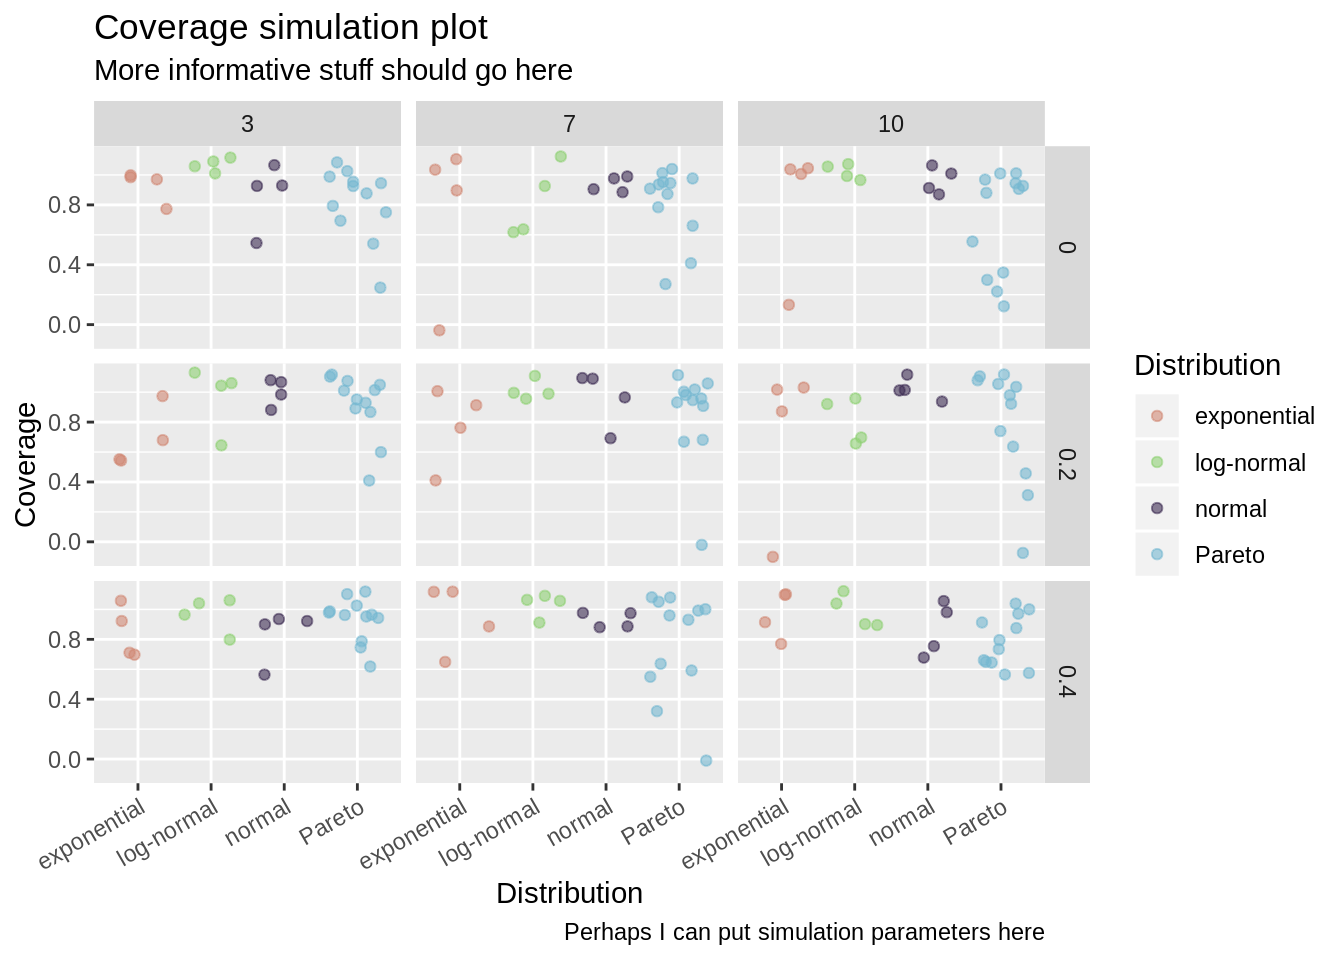
\includegraphics[width=\textwidth]{placeholder-coverage-plot.png}
   \caption{Simulation results.}
   %\label{fig:sims}
\end{figure}




\section{Meta-analysis of medians}

Our motivating problem was meta-analysis of medians, and we have followed the \emph{toolchain walkthrough}~\cite{gray2019textttcodeproof} for computationally developing a statistical estimator. This process took us from mathematical derivations, to estimator functions provided by \emph{research compendia}~\cite{grayTruthProofReproducibility2019} \package{varameta}~\cite{grayVarametaEstimatorsVariance2020}, to \emph{coverage probability} simulations provided by the package \package{simeta}~\cite{graySimetaSimulateMetaanalysis2020} to explore the efficacy of this estimator under different sampling conditions. In so doing, this manuscript raises the question if examining research software engineering methodology, of exploring the efficacy of an estimator, in the context of rapidly evolving statistical tools for simulation and analysis, is of research merit in its own right. We begin by revisiting our motivating example, and turn to metaresearch observations from this analysis.

\subsection{Revisiting the motivating example}
\label{sec: pin again}

With a method for incorporating medians, we revisit the meta-analysis presented by Pinheiro \emph{et al.}\dothislater{Remember to replace the tired old Pinheiro example}.

\morewords{Figure: forest plot}
\morewords{paused for writing tracking}



\subsection{Components of research for computational science}

\morewords{It is not immediately apparent what the best way to confer analyses.}

\morewords{metaresearch context}

This manuscript derives mathematical estimators and presents simulation results of programmed instantiations of the algorithmic solution to the meta-analysis of medians. Rapid advances in the adoption software engineering provide an auxillary context of metaresearch; these are explored in companion manuscripts that describe the theoretical underpinnings of reproducible computing~\cite{grayTruthProofReproducibility2019} and the practical steps in preparing this analysis as a reproducible research compendium~\cite{gray2019textttcodeproof}. Which is to say, metaresearch questions from this project have generated more products of research than the question of meta-analysing medians itself.

This manuscript is one product of a research question. However, against the backdrop of technological revolutions in data collection and code sharing, contemporary researchers face a constant challenge of upskilling in computational tools, in addition to the challenges of the discipline in which the researcher is working. This manuscript used two packages, \package{varameta} and \package{simeta} to perform analysis; this manuscript is but one research component of the compendium of research to assess estimators for meta-analysis of medians. This splintered approach has the advantage that each component can exist for a different utility, individually, but together form a compendium of research.

Sharing and reflecting on how we do this can surely be of benefit to others, especially for those with the leisure to learn new techniques, such as graduate students.

%%% Bibliography

\medskip
\printbibliography


\end{document}
